\section{Design}
\label{s:gen}

This section describes \sys's design for constraint generation and
solving.

\subsection{Basic Architecture}

\sys's constraint generator is implemented as a set of compiler
passes in the LLVM~\cite{lattner:llvm} framework.  The workflow is
shown in \autoref{f:flow}.  The error and path constraint generation
passes work on LLVM intermediate representations, which are compiled
from source code with all optimizations turned off.  They inspect
one function at a time, so as to bound the size of constraints.

To improve the accuracy, \sys allows users to annotate the ranges
of variables, such as function parameters and structure fields, as
additional constraints. It also employs a whole-program pass that
infers the range constraints across the call graph.

\begin{figure}
\centering
\resizebox{0.9\linewidth}{!}{
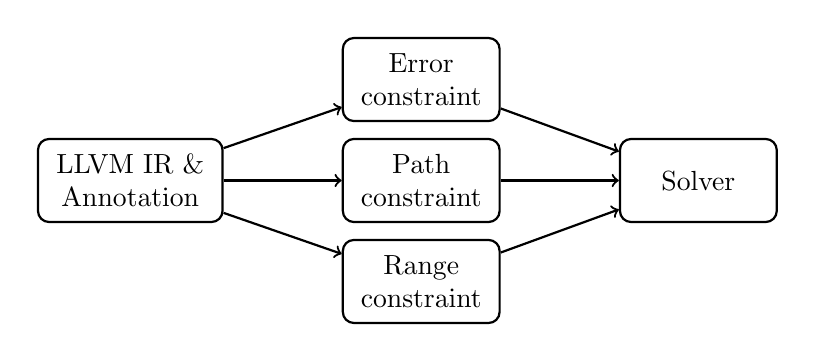
\begin{tikzpicture}[
	block/.style={
		rectangle, rounded corners,
		draw=black, thick,
		text width=5em, minimum height=3em, text centered
	},
	line/.style={draw, thick, ->},
	]
	\matrix[row sep=2mm, column sep=15mm] {
		& \node [block] (ec) {Error constraint}; & \\
		\node [block, text width=6em] (ir) {LLVM IR \& Annotation};
		& \node [block] (pc) {Path constraint};
		& \node [block] (sol) {Solver}; \\
		& \node [block] (rc) {Range constraint}; & \\
	};

	\path [line] (ir) -- (ec);
	\path [line] (ir) -- (pc);
	\path [line] (ir) -- (rc);
	\path [line] (ec) -- (sol);
	\path [line] (pc) -- (sol);
	\path [line] (rc) -- (sol);
\end{tikzpicture}

}
\caption{\sys's worflow.}
\label{f:flow}
\end{figure}

\subsection{Error Constraint Generation}

%Size/alloc/index annotation.

Constant folding.

Pointer arithmetic simplification.
- symbolic~\cite{engelen:symbolic}.

Integer operation sinking.

Checking idiom recognition.

Load hoisting.

\subsection{Path Constraint Generation}

Error constraint generation.
- Loop constraint generation.

Path constraint generation.

\subsection{Value Range Inference}

Range constraint \& annotations?

\subsection{Limitations}

miss bugs in some configurations, architectures,
and assembly code.
